\documentclass[a4paper]{article}
\usepackage[italian]{babel}
\usepackage[T1]{fontenc}
\usepackage[utf8]{inputenc}
\usepackage{graphicx}
\usepackage{float}

\begin{document}

\begin{figure}
	\begin{center}
    	
\includegraphics[scale=0.6]{Immagini/FedericoII}
    \end{center}
\end{figure}

\title{PROGETTAZIONE E SVILUPPO DI UN DATABASE PER LA 
    	   GESTIONE DI UNA GALLERIA FOTOGRAFICA}
\author{Ciro Pizza - N86004131\\ Vincenzo Riccardo - N86004134\\ Salvatore Savino - N86004099}
\maketitle

\newpage
\tableofcontents
\newpage

\section{INTRODUZIONE}
\vspace{12pt}
	Lo scopo di questo progetto è lo sviluppo di un sistema
	informativo per la \textbf{gestione di collezioni
	fotografiche condivise}. Il sistema sarà
	implementato 
	attraverso un database ed un'applicazione Java
	dotata di GUI, realizzata con
	la tecnologia JavaFX. In particolare, per il sistema è
	richiesto che
	ogni fotografia
	dovrà contenere informazioni sull'utente che l'ha
	scattata, il dispositivo utilizzato, il luogo di scatto
	(identificato da coordinate geografiche o da un nome
	mnemonico unico) e i soggetti che la caratterizzano. Il
	sistema consentirà dunque agli utenti di caricare e
	visualizzare tali fotografie, fornendo
	anche filtri di ricerca delle immagini in base al
	loro luogo e al loro soggetto.
	Funzionalità importanti dovranno essere quelle che
	permettono
	all'utente di creare video
	(una semplice sequenza di alcune sue foto) e
	quella di partecipare a delle
	collezioni condivise con altri utenti, in cui possono
	essere raggruppate sia le proprie foto sia quelle degli
	altri partecipanti. Inoltre, gli utenti avranno sia la
	possibilità di gestire la "privacy" delle
	proprie foto (rendendole cosi esclusivamente personali e
	quindi non condivisibili), sia
	di eliminarle in qualsiasi momento (rendendole cosi
	non più disponibili nella propria galleria personale,
	senza
	però cancellarle definitivamente dal sistema qualora
	fossero presenti in delle collezione condivise). Infine,
	a
	gestione dell'utenza, dovrà esserci un amministratore con 
	la facoltà di poter eliminare gli utenti dal sistema;
	all'eliminazione di un utente dovranno naturalmente
	essere cancellate
	tutte le sue foto dal sistema, eccetto quelle che
	contengono come soggetto un altro degli utenti della
	galleria condivisa in cui la foto è presente.
	\\\\
	In questo documento andremo a trattare il progetto dal
	punto di vista della base di dati. Per realizzarla, è
	stato utilizzato un database relazionale sviluppato
	grazie al \textbf{DBMS Postgre}. Il sistema è stato
	progettato con
	particolare attenzione alla semplicità, alla
	facilità d'uso e
	all'intuitività dell'interfaccia grafica, al fine
	di
	rendere l'esperienza dell'utente il più piacevole e
	soddisfacente possibile. Verrà presentato il progetto nel
	dettaglio, a partire dalla scelta delle entità e degli
	attributi, passando per il diagramma ER e quello UML,
	fino ad arrivare alla scelta dello schema logico e alla
	descrizione delle varie funzionalità del sistema,
	implementate attraverso procedure, funzioni e
	trigger.



\vspace{45pt}
\section{PROGETTAZIONE CONCETTUALE}
	\vspace{12pt}
	\subsection{Analisi dei Requisiti}
	\vspace{8pt}
	Per la realizzazione del database relazionale richiesto,
	abbiamo innanzitutto bisogno di individuare i "concetti"
	del nostro \textbf{mini-world}, che useremo poi per
	andare a
	creare un  diagramma completo; inizieremo rappresentando
	questi concetti di base attraverso \emph{entità} ed
	\emph{attributi}
	del
	\textbf{modello ER} (entità-relazione), essendo
	abbastanza
	intuitivo e di facile comprensione. Al centro del
	problema, c'è
	sicuramente il concetto (in questo caso, l'entità)
	\framebox{\textbf{FOTOGRAFIA}}, senza il quale
	ovviamente non si potrebbe parlare di "galleria
	fotografica". Per la nostra fotografia, si va allora ad
	indicare
	il suo \textbf{valore} (che può essere ad esempio il suo
	path all'interno del computer),
	il \textbf{dispositivo} con il quale è stata scattata
	(specificando anche alcune sue caratteristiche) e il
	\textbf{luogo} in
	cui è stata scattata. La fotografia deve
	essere stata sicuramente scattata da un \textbf{utente}
	(che ne è
	naturalmente anche il "proprietario"), e può anche
	contenere diverse categorie di
	\textbf{soggetti} che la raffigurano (ndr: \emph{un
	utente può
	essere
	esso stesso un soggetto, quindi lo si va a
	specificare}). La fotografia può inoltre essere parte di
	diversi \textbf{video}, ed essere inserita in svariate
	\textbf{collezioni}.
	Infine, sfruttando il \textbf{modello EER}
	(Enhanced ER) per
	modellare il nostro miniworld in maniera ancora più
	dettagliata, si è specificato, attraverso delle
	sottoclassi, che la foto può essere \textbf{privata}
	(ovvero disponibile solo a sè stessi) o
	\textbf{pubblica} (quindi condivisibile con altre
	persone), ma
	anche \textbf{eliminata}
	(inserita in una sorta di cestino) o \textbf{non
	eliminata}
	(visibile tranquillamente nella propria galleria
	personale). 
	Si ricorda, inoltre, che gli attributi
	multivalore vengono indicati con
	due cerchi concentrici, mentre, per quanto
	riguarda l'EER, si indica il
	\textbf{vincolo di disgiunzione} con una \textbf{"d"} per
	specificare 
	che una
	singola foto può essere membro di \emph{al massimo} una
	sottoclasse, e il \textbf{vincolo di
	completezza
	totale}
	con una doppia linea per specificare che ogni foto deve
	essere \emph{necessariamente} membro di qualche sua
	sottoclasse.

	\begin{figure}[H]
        \begin{center}
            \includegraphics[scale=0.25]{Immagini/entità_fotografia}
            \caption{Entità FOTOGRAFIA}
        \end{center}
	\end{figure}

	\vspace{10pt}
	Partendo da qui, sicuramente si ha la strada spianata
	per "scovare" 
	tutte le altre entità. Si è subito
	pensato
	all'entità \framebox{\textbf{LUOGO}}, specificato
	semplicemente dal
	nome di una \textbf{città}, e
	che ovviamente può essere presente in più di una
	\textbf{fotografia}, e all'entità
	\framebox{\textbf{VIDEO}},
	creato da un \textbf{utente} e
	sequenza di più \textbf{fotografie}. Per il video si è
	inserita la possibilità di poter aggiungere una breve
	\textbf{descrizione}, utile eventualmente per descriverne
	il suo contenuto.

	\begin{figure}[H]
        \begin{center}
            \includegraphics[scale=0.25]{Immagini/entità_luogo}
            \caption{Entità LUOGO}
        \end{center}
	\end{figure}
	
	\vspace{8pt}

	\begin{figure}[H]
        \begin{center}
            \includegraphics[scale=0.25]{Immagini/entità_video}
        \caption{Entità VIDEO}
        \end{center}
	\end{figure}

	\vspace{9pt}
	Altra entità che si è presa in
	considerazione è la \framebox{\textbf{COLLEZIONE}},
	raggruppamento di una o
	più \textbf{fotografie}, e
	dunque fulcro del nostro sistema. Da notare che, cosi
	come può avere più foto, una singola collezione può
	anche essere "posseduta" da più \textbf{utenti} che
	vogliono poter
	condividere le loro foto; di conseguenza, si può anche 
	qui sfruttare il modello EER per specificare due diverse
	sottoclassi di collezioni: \textbf{personale}, ad
	indicare la collezione di default a cui ha accesso
	esclusivamente il singolo 		
	utente, composta quindi dalle sole foto caricate /
	scattate da lui, e \textbf{condivisa}, ad indicare il
	fatto che la collezione in questione è stata creata in
	seguito da più utenti
	(partecipanti ad essa), e che può dunque essere formata
	da fotografie provenienti da diversi utenti. Inoltre, per
	quanto riguarda la collezione
	condivisa, si è pensato alla possibilità di farla
	assegnare, al momento della sua reazione, un
	\textbf{nominativo}
	per poterla riconoscere. 

	\begin{figure}[H]
        \begin{center}
            \includegraphics[scale=0.24]{Immagini/entità_collezione}
            \caption{Entità COLLEZIONE}
        \end{center}
	\end{figure}

	\vspace{10pt}
	Arrivati a questo punto, si può sicuramente notare che
	COLLEZIONE,
	FOTOGRAFIA e
	VIDEO non possono esistere senza un determinato utente
	che li
	possegga, li scatta e li crea. Di conseguenza,
	non può mancare l'entità \framebox{\textbf{UTENTE}};
	si può descrivere quest'ultima con delle \textbf{informazioni
	personali}
	(come nome, cognome ecc...) e delle \textbf{credenziali}
	(come
	e-mail e password) con il quale può accedere univocamente
	al sistema.

	\begin{figure}[H]
        \begin{center}
            \includegraphics[scale=0.25]{Immagini/entità_utente}
            \caption{Entità UTENTE}
        \end{center}
	\end{figure}

	\vspace{10pt}
	Infine, dato che a gestione degli stessi \textbf{utenti}
	è
	richiesto un
	amministratore con facoltà di poterli eliminare in
	qualsiasi momento, si è pensato, come
	ultima entità, all'\framebox{\textbf{AMMINISTRATORE DEL
	SISTEMA}},
	una
	sorta
	di
	"superutente" che non ha bisogno di specifiche
	informazioni personali, ma per cui basta e
	avanza una speciale \textbf{password} d'accesso.
	
	\begin{figure}[H]
        \begin{center}
            \includegraphics[scale=0.25]{Immagini/entità_amministratore}
            \caption{Entità AMMINISTRATORE DEL SISTEMA}
        \end{center}
	\end{figure}



	\vspace{35pt}
	\subsection{ER Diagram}
	\vspace{8pt}
	Una volta trovate le varie astrazioni del nostro 
	mini-world, e modificate intuitivamente in entità
	con relativi attributi, si può facilmente notare che
	esistono numerosi\emph{ rapporti impliciti} che
	intercorrono tra loro:

	\begin{itemize}
		\item L'attributo \emph{Utenti} di AMMINISTRATORE si
		riferisce all'entità
		UTENTE
		\item Gli attributi \emph{Collezioni},
		\emph{Fotografie}
		e \emph{Video} di UTENTE si riferiscono alle
		rispettive
		entità COLLEZIONE, FOTOGRAFIA e VIDEO
		\item e cosi via\dots
	\end{itemize}
	
	Inizialmente si possono rappresentare questi rapporti
	come attributi, ma, in un modello ER che si rispetti,
	occorre invece trasformarli in delle
	\textbf{relazioni}, con rispettive \textbf{cardinalità}.
	Di
	conseguenza, un volta effettuato questo passaggio,
	ci si ritrova
	con il seguente ER diagram finale:
	\vspace{5pt}
	
	\begin{figure}[H]
        \begin{center}
            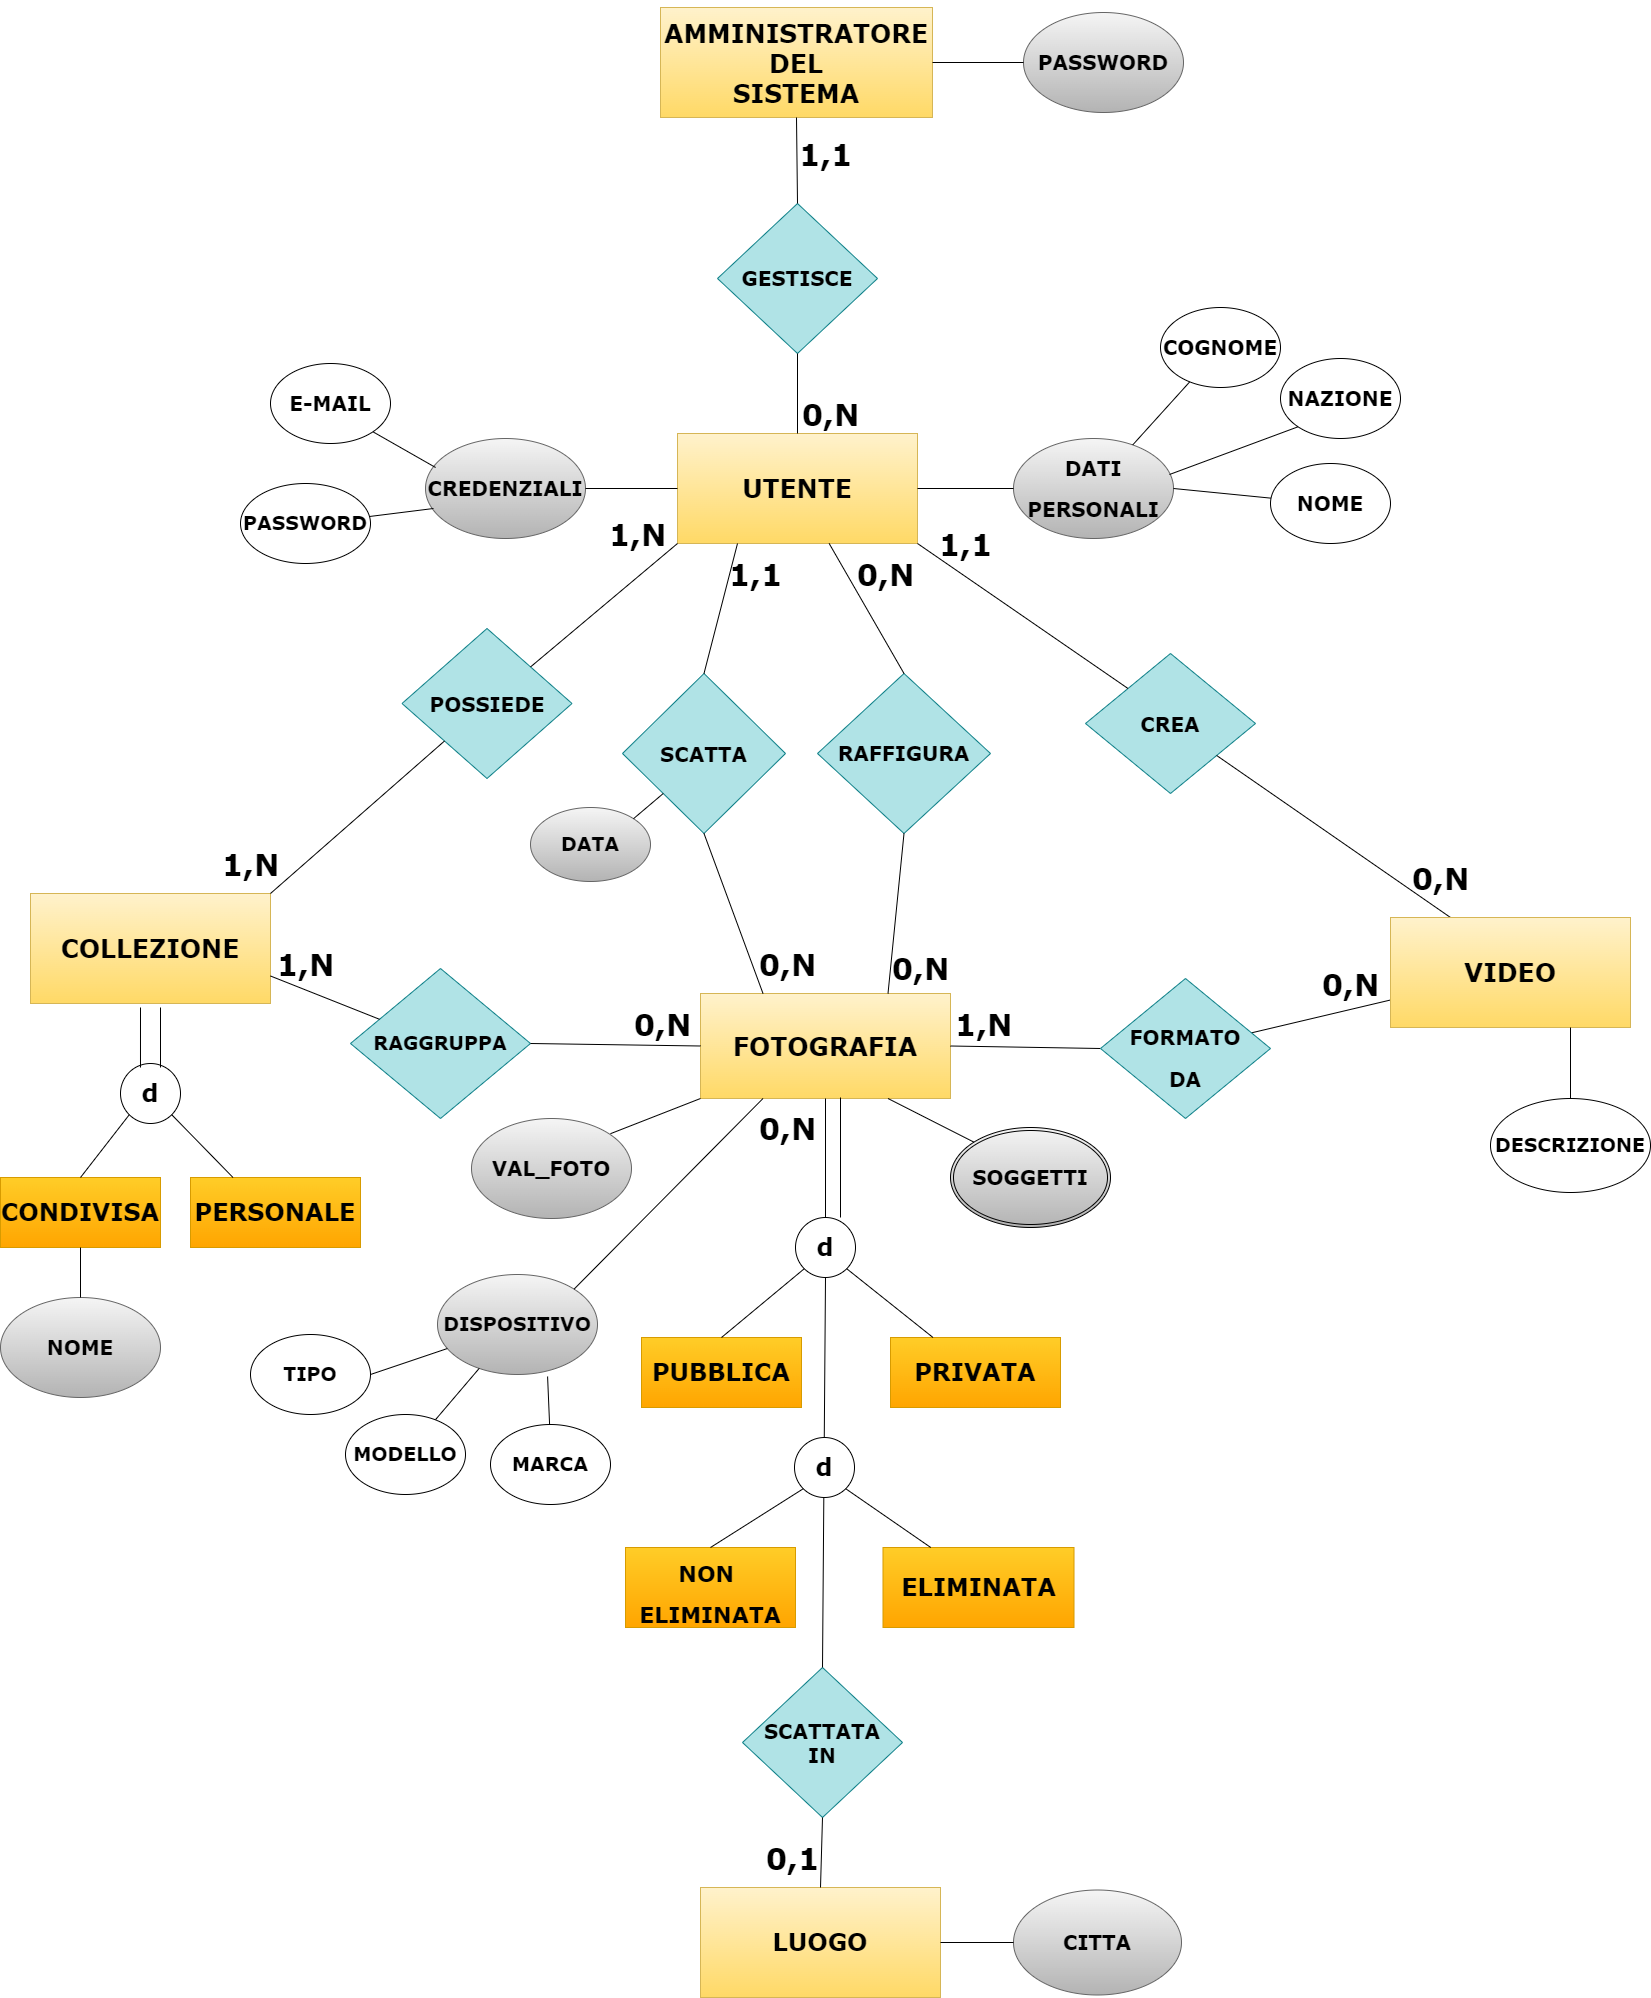
\includegraphics[scale=0.24]{Immagini/Galleria_Fotografica_ER}
        	\caption{ER Diagram}
        \end{center}
	\end{figure}



	\vspace{35pt}
	\subsection{Class Diagram}
	\vspace{8pt}
	Completato il diagramma ER, si è  poi optato,
	soprattutto per questione di praticità e compatibilità
	col modello a oggetti di JAVA, alla trasformazione di
	quest'ultimo in un\textbf{ Class Diagram UML},
	sostituendo le
	entità con le \textbf{classi}, e le relazioni con le
	\textbf{associazioni}:
	
		\begin{figure}[H]
        \begin{center}
            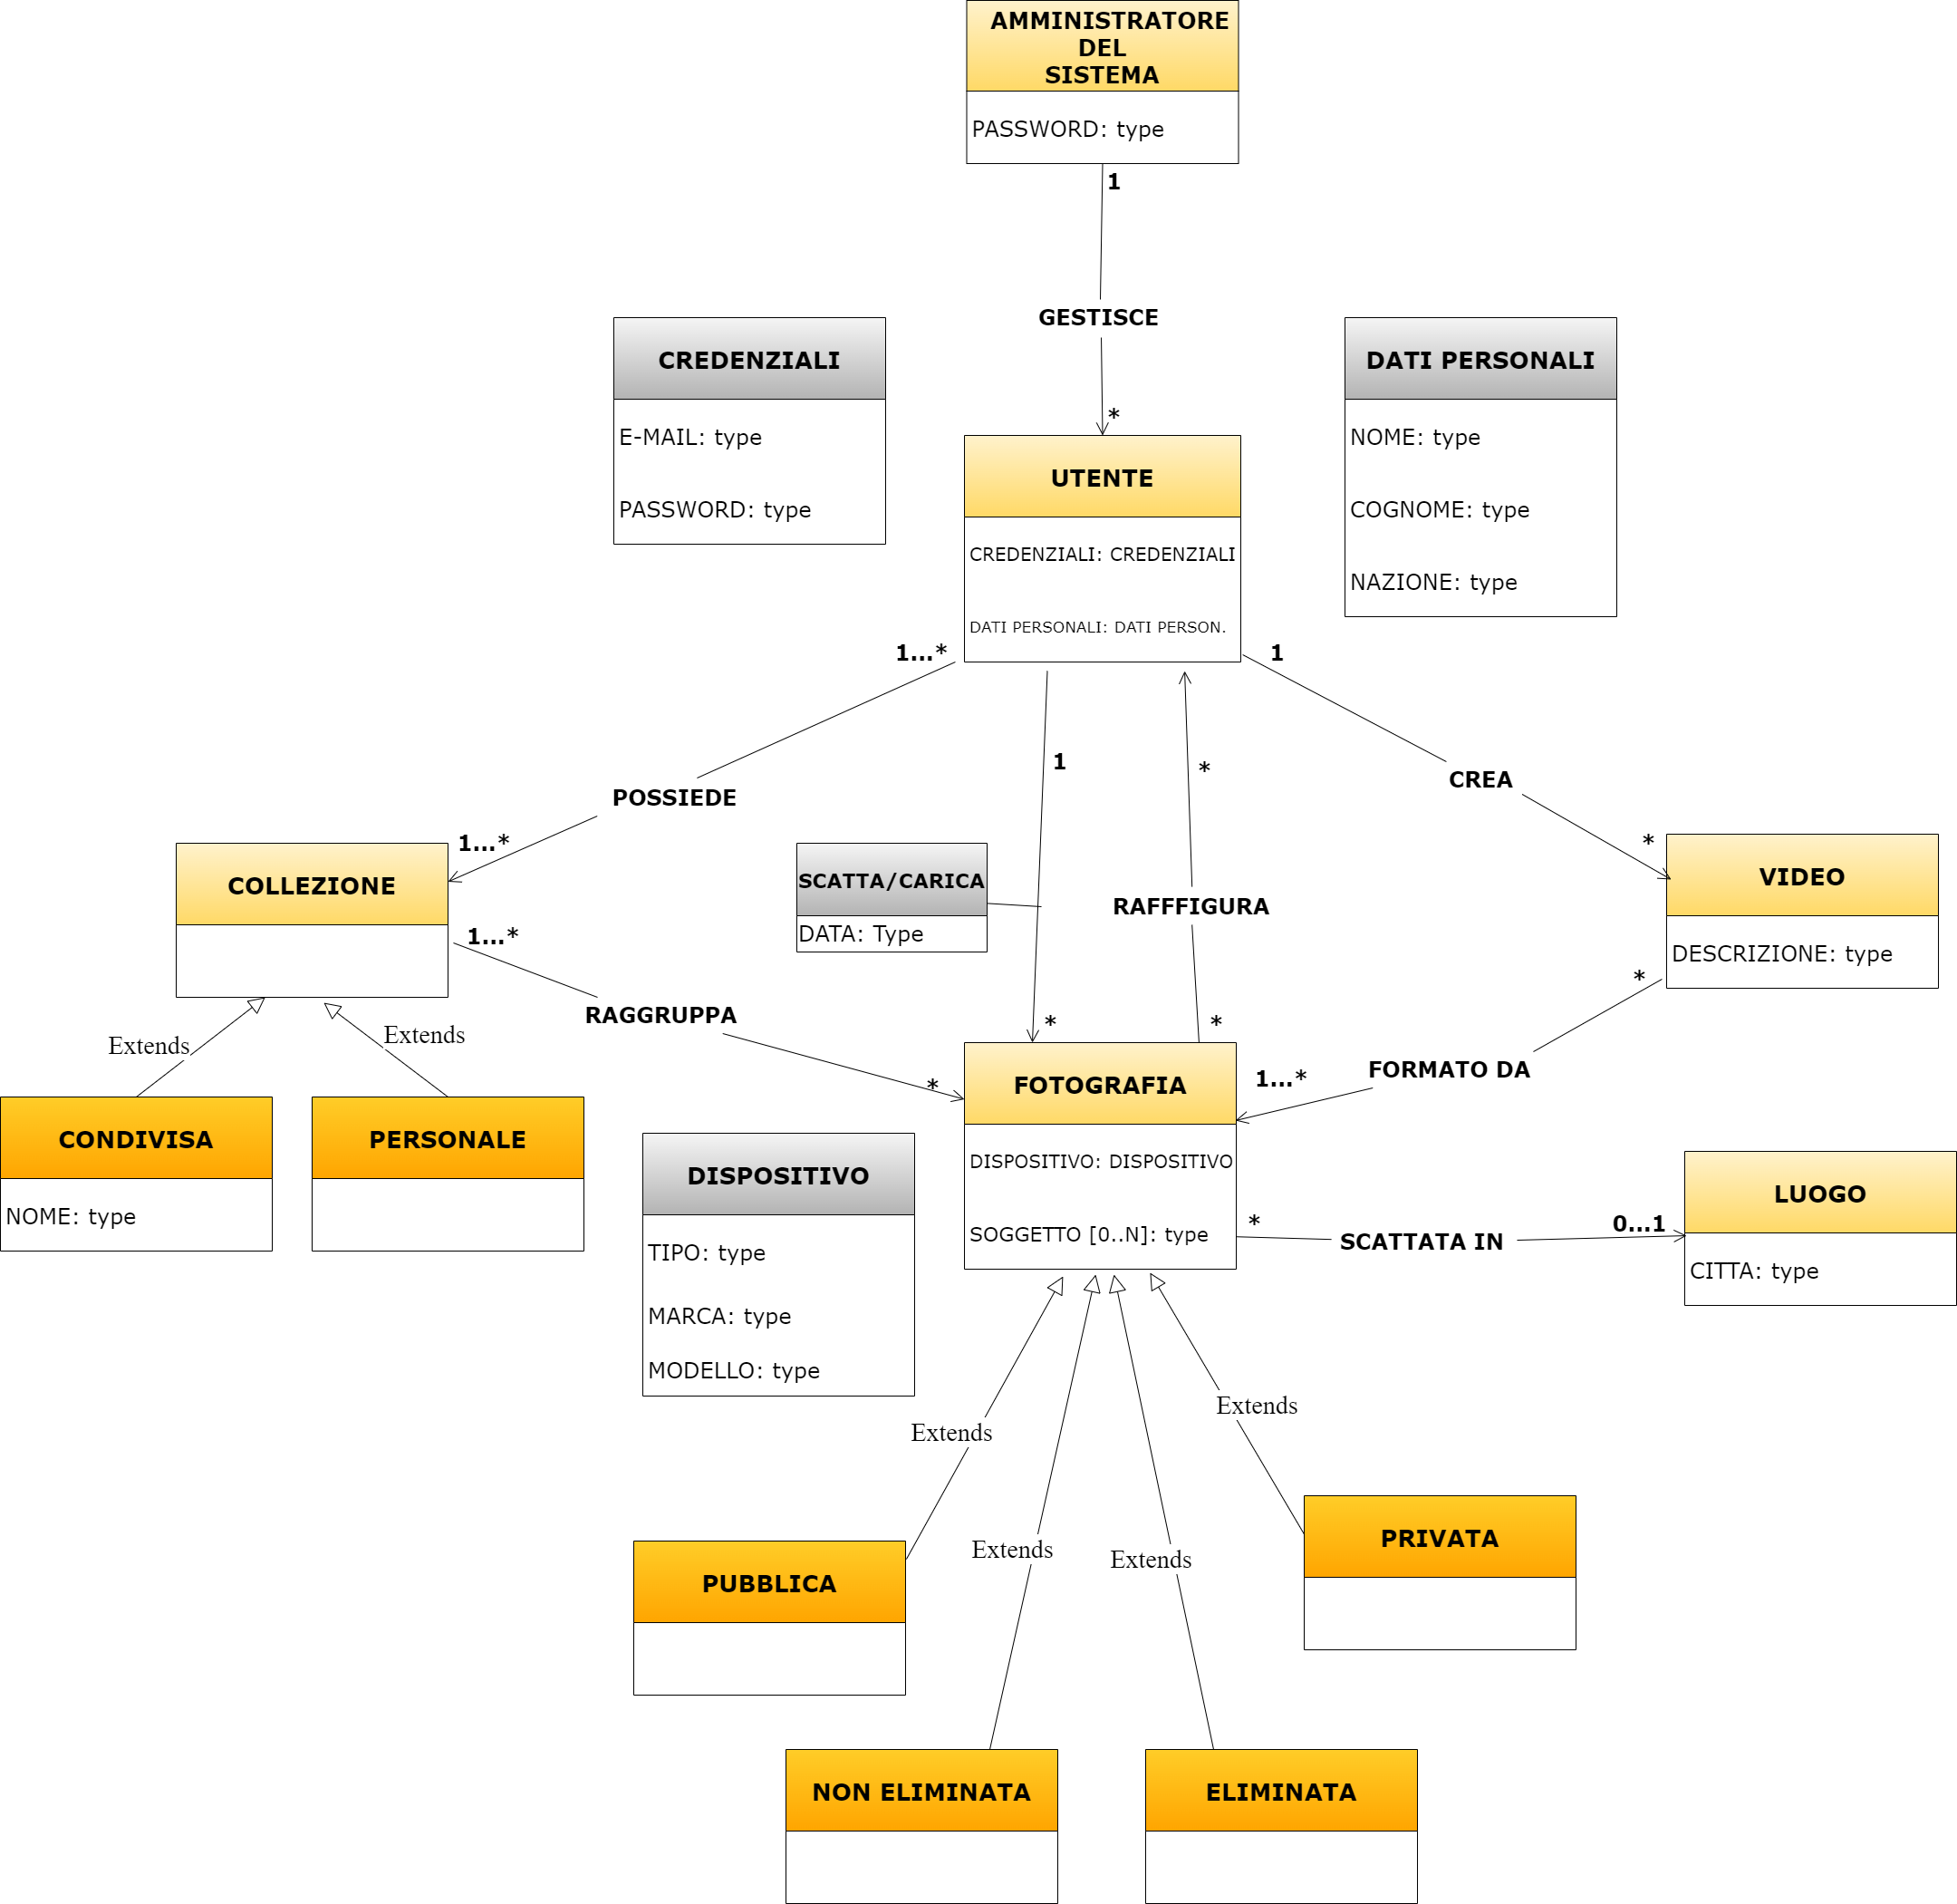
\includegraphics[scale=0.20]{Immagini/Galleria_Fotografica_UML}
            \caption{Class Diagram UML}
        \end{center}
	\end{figure}
	Si può notare che, in questo determinato frangente,
	si è deciso di lasciare intenzionalmente
	il valore dei tipi degli attributi come \emph{"type"},
	inteso come un tipo non ancora specificato.
	
	
	
	\vspace{35pt}
	\subsection{Analisi di ristrutturazione del Class Diagram}
	\vspace{8pt}
	Non tutti i costrutti che si sono utilizzati nei
	precedenti
	diagrammi hanno una traduzione naturale nei modelli
	logici che saranno poi implementati nei database
	relazionali; dunque,
	al fine di rendere il nostro Class Diagram idoneo, e per
	migliorare l’efficienza generale dell’implementazione, si
	procede alla sua \textbf{ristrutturazione}. La fase di
	ristrutturazione di uno schema concettuale è suddiviso
	generalmente in:
	
	\begin{enumerate}
		\item Analisi delle ridondanze
		\item Eliminazione delle Generalizzazioni
		\item Eliminazione Attributi Multipli
		\item Eliminazione Attributi Strutturati
		\item Partizionamento/Accorpamento di classi e
			  associazioni
		\item Analisi degli Identificativi
	\end{enumerate}

	\vspace{20pt}
		\subsubsection{Analisi delle Ridondanze}
		\vspace{5pt}
		Non si sono rilevate particolari ridondanze nel
		Class Diagram.
		
		\vspace{20pt}
		\subsubsection{Eliminazione delle Generalizzazioni}
		\vspace{5pt}
		Sono presenti ben due generalizzazioni nel
		Class Diagram: COLLEZIONI e FOTOGRAFIA, con le loro
		rispettive sottoclassi. Si ricorda che entrambe le
		classi generalizzate hanno un \textbf{vincolo
		di specializzazione totale}, e dunque, per poterle
		eliminare, la scelta più opportuna è sicuramente
		quella di applicare una delle seguenti opzioni:
		
		\begin{itemize}
			\item[a)] Accorpamento delle figlie della
			generalizzazione nel padre
			\item[b)] Accorpamento del padre della
			generalizzazione nelle figlie
		\end{itemize}
		Si è optato alla fine per la scelta \textbf{a)},
		considerando soprattutto che:
		
		\begin{itemize}
			\item Le classi di specializzazioni non hanno
			particolari attributi che li distinguono tra loro
			(nel caso di FOTOGRAFIA ne abbiamo addirittura 0) 
			\item Le operazioni che andremo a fare su classe
			padre e classi figlie sono  praticamente le
			stesse
		\end{itemize}
		All'interno della classe COLLEZIONE sono stati cosi
		aggiunti l'attributo \emph{nome} (appartenente alla
		vecchia
		sottoclasse CONDIVISA),
		e
		l'attributo
		\emph{personale} (flag a cui verrà assegnato un
		semplice
		valore intero, 0 od 1, utile
		distinguere le due ex sottoclassi implicite). Nella
		classe FOTOGRAFIA vengono aggiunti invece
		gli attributi \emph{pubblica} ed \emph{eliminata},
		che
		hanno
		la medesima funzionalità di
		\emph{personale}.
		Si è dunque evitato di introdurre più classi,
		ottenendo sicuramente un \textbf{minor numero di
		accessi}, con l'unica trascurabile pecca di
		introdurre dei valori nulli nel caso una collezione
		sia \emph{personale} (ndr: una collezione personale
		non ha un nome).
		
		\vspace{20pt}
		\subsubsection{Eliminazione degli Attributi Multipli}
		\vspace{5pt}
		È presente un unico attributo multivalore, ovvero
		\emph{soggetti} (FOTOGRAFIA). Per eliminarlo, tra le
		tecniche a disposizione che si possono sfruttare,
		ovvero: 

		\begin{itemize}
			\item[a)] Creare una entità esterna associata
			\item[b)] Trattare l'attributo come singolo
			\item[c)] Replicare l'attributo nella classe
		\end{itemize}
		Si è optato alla fine per la\textbf{ creazione di una
		entità esterna associata}, con l'aggiunta
		dell'attributo
		\emph{categoria} che va a specificare il tipo di
		soggetto in
		questione. La scelta è giustificata
		dal fatto che, avendo l'idea di inizializzare il
		database con diversi \textbf{soggetti di default}, si
		è ritenuto
		molto utile avere una determinata classe
		in
		cui
		poterli
		"immagazzinare". Inoltre, si è considerato abbastanza
		sprecato sia trattare l'attributo
		come se fosse singolo (riducendo ad una foto la
		possibilità di avere diversi soggetti), sia
		replicarlo all'interno della classe (rischiando cosi
		di avere eccessivi valori nulli).

		\vspace{20pt}	
		\subsubsection{Eliminazione degli Attributi Strutturati}
		\vspace{5pt}
		Per quanto riguarda gli attributi strutturati, ne
		sono presenti tre: \emph{credenziali} (UTENTE),\emph{
		dati personali} (UTENTE) e \emph{dispositivo}
		(FOTOGRAFIA). Anche qui, come nel caso degli
		attributi multipli, si può ricorrere a 3 modi per
		eliminarli:
		
		\begin{itemize}
			\item[a)] Introduzione di una classe
			\item[b)] Estrazione degli attributi
			\item[c)] Eliminazione degli attributi
		\end{itemize}
		Non si è ritenuto nessun attributo all'altezza di
		avere una specifica classe. Si è invece optato,
		per l'attributo \emph{dispositivo},
		ad una netta \textbf{eliminazione} dei suoi
		attributi, considerati abbastanza superflui per le
		funzionalità del
		progetto, mentre, per quanto riguarda
		\emph{dati personali} e \emph{credenziali}, alla loro
		\textbf{estrazione} nella classe UTENTE, essendo
		valutati entrambi di notevole importanza.
		
		\vspace{20pt}		    
        \subsubsection{Partizione/Accorpamento di classi e associazioni}
        \vspace{5pt}
        Non sono stati individuate particolari
        classi che
        necessitano di un'eventuale partizione o
        accorpamento. Si era inizialmente pensato, per
        una questione di maggior praticità, ad
        accorpare la classe LUOGO alla classe FOTOGRAFIA, sia
        considerando
        il fatto che LUOGO avesse un solo attributo, sia
        considerando
        il potenziale
       	numero elevato di città/località da dover
       	immagazzinare in essa (molto maggiore
       	rispetto alle categorie dei soggetti, ad esempio).
       	Però, per rispettare la richiesta di avere
       	ogni
       	luogo identificato univocamente, si è deciso alla
       	fine di
       	rimanere con la classe LUOGO. Per quanto riguarda le
       	associazioni, si è deciso invece di accorpare
       	l'attributo
       	dell'associazione
       \textbf{\emph{"scatta"}}, ovvero \emph{data}, nella
       classe
       FOTOGRAFIA.
       	
        \vspace{20pt}		    
        \subsubsection{Analisi degli identificativi}
        \vspace{5pt}
        Infine, per quanto riguarda la scelta degli
        identificativi
        del Class Diagram, si è optato per i
        seguenti attributi:
        
        \begin{itemize}
        	\item \emph{ID\textunderscore amminist}
        	(AMMINISTRATORE DEL SISTEMA)
        	\item \emph{ID\textunderscore utente},
        	\emph{email} (UTENTE)
        	\item \emph{ID\textunderscore foto}
        	(FOTOGRAFIA)
        	\item \emph{ID\textunderscore collezione},
        	\emph{nome} (COLLEZIONE)
        	\item \emph{ID\textunderscore video} (VIDEO)
        	\item \emph{ID\textunderscore soggetto},
        	\emph{categoria} (SOGGETTO)
        	\item \emph{città} (LUOGO)
        \end{itemize}
        Da come si può notare, si è scelto di identificare
        ogni classe, ad eccezione di LUOGO (per cui si è
        pensato sufficiente l'attributo \emph{città}), con
        uno
        specifico
        attributo di \textbf{chiave primaria} in cui nel nome
        è incluso il prefisso "\textbf{ID}". Ci sono poi tre
        \textbf{chiavi secondarie}, anch'esse uniche
        all'interno del sistema, ovvero \emph{email}
        (UTENTE), \emph{nome} (COLLEZIONE) e \emph{categoria}
        (SOGGETTO). Per quanto riguarda \emph{email}, è
        abbastanza scontato il fatto che, per questione di
        univocità, due utenti non possano avere una stesso
        indirizzo di posta elettronica. Per quanto riguarda
        \emph{categoria}, anche qui è abbastanza intuitivo il
        fatto che è assolutamente inutile avere due tipologie
        di soggetto uguali all'interno della stessa classe.
        Infine, per quanto riguarda il \emph{nome} della
        collezione, pur essendo in teoria assolutamente
        concepibile avere due nomi uguali all'interno del
        sistema, si è deciso di usarla come chiave
        semplicemente per una questione di praticità,
        rendendo la ricerca più semplice da gestire
        all'interno dell'applicativo JAVA.
        
        \newpage
        

    \subsection{Class Diagram Ristrutturato}
    \vspace{8pt}
	Completata la ristrutturazione, ci si ritrova infine con
	il seguente Class Diagram:
	
	\begin{figure}[H]
        \begin{center}
            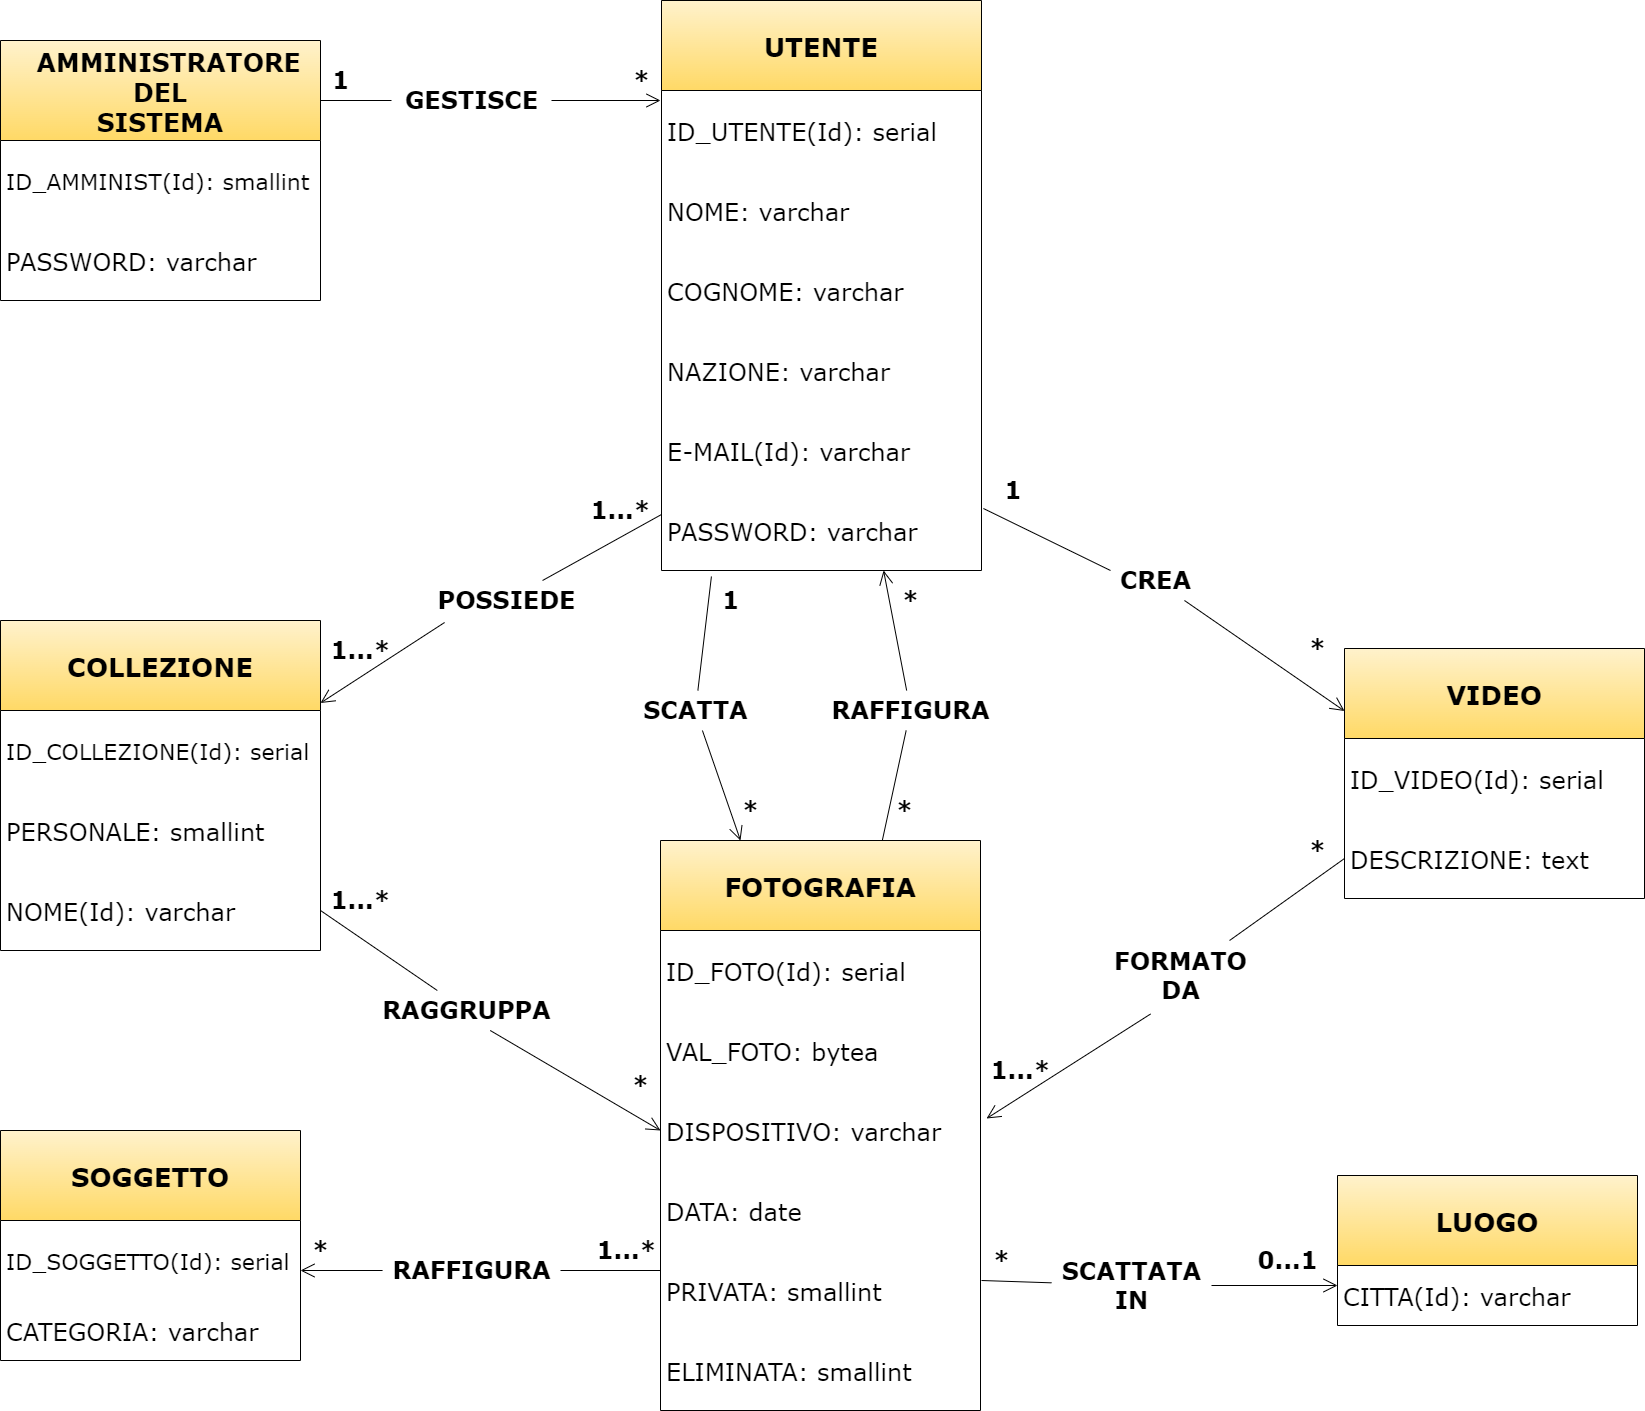
\includegraphics[scale=0.20]{Immagini/Galleria_Fotografica_UML_Ristrutturato}
            \caption{Class Diagram UML - Ristrutturato}
        \end{center}
	\end{figure}

Si può notare che, in questo frangente, sono stati specificati tutti i tipi che saranno poi assegnati agli attributi al momento dell'implementazione definitiva. Inoltre, si sottolinea che a tutte le chiavi con prefisso
\emph{"ID"} (eccetto \emph{id\textunderscore amminist}, che non ne ha bisogno) è
stato assegnato il tipo
\textbf{serial}. Quest'ultimo, in Postgre, non è altro che un intero con aumento automatico del proprio valore ad ogni inserimento di una nuova tupla,  caratterizzato da un \textbf{valore iniziale} e da un \textbf{incremento} impostati e gestiti a nostra preferenza.



\vspace{35pt}
\section{DIZIONARIO DELLE CLASSI, DELLE ASSOCIAZIONI e DEI VINCOLI}
\vspace{5pt}
	Andremo ora a vedere, nel dettaglio,
	attraverso un \textbf{dizionario} in formato tabellare,
	tutte le classi, le associazioni e i vincoli coinvolte
	nel nostro
	Class Diagram. 
	
	\vspace{12pt}
	\subsection{Dizionario delle Classi}
	\vspace{8pt}
	\begin{tabular}{p{90pt}p{120pt}p{150pt}}
		\hline
		\textbf{Classe} & \textbf{Descrizione} & 
		\textbf{Attributi} 
		\\
		\hline
		\hline
		\hline
		
		\textbf{Amministratore del Sistema} &
		Classe che rappresenta il responsabile del sistema,
		incaricato alla gestione dell'utenza &
		\textbf{ID\textunderscore amminist}
		(\emph{smallint}):
		chiave
		primaria della classe che identifica univocamente
		l'amministratore.\newline 
		\textbf{Password} (\emph{varchar}): stringa d'accesso
		all'esclusiva sezione di gestione
		dell'amministratore. 
		\\
		\hline
		
		\textbf{Utente} &
		Classe che rappresenta i clienti utilizzatori della
		galleria fotografica &
		\textbf{ID\textunderscore utente} (\emph{serial}):
		chiave
		primaria della classe che identifica univocamente
		ogni singolo utente. Il suo valore iniziale è
		impostato
		ad 1, cosi come il suo incremento.\newline 
		\textbf{Nome} (\emph{varchar}): nome dell'utente.
		\newline 
		\textbf{Cognome} (\emph{varchar}): cognome
		dell'utente.
		\newline
		\textbf{Nazione} (\emph{varchar}): nazione d'origine
		dell'utente.
		\newline
		\textbf{Email} (\emph{varchar}): chiave secondaria
		della classe, specifica l'indirizzo di posta
		elettronica dell'utente.\newline
		\textbf{Password} (\emph{varchar}): stringa che
		permetta all'utente di accedere al sistema.
		\\
		\hline
		
		\textbf{Fotografia} &
		Classe che rappresenta le fotografie &
		\textbf{ID\textunderscore foto} (\emph{serial}):
		chiave
		primaria della classe che identifica univocamente
		ogni singola fotografia. Il suo valore iniziale è
		impostato
		a 100, mentre il suo incremento ad 1. \newline 
		\textbf{Val\textunderscore foto} (\emph{bytea}):
		valore
		della fotografia, inteso come la rappresentazione che
		ha la foto all'interno del database. Si è preferito
		assegnargli il tipo bytea (il binary string di
		Postgre, simile al BLOB), andando cosi a memorizzare
		i byte della foto direttamente nel database.\newline
		\textbf{Dispositivo} (\emph{varchar}): dispositivo
		con
		il quale è stata scattata la foto.\newline 
		\textbf{Data} (\emph{date}): data in cui la foto è
		stata caricata nel sistema.\newline 
		\textbf{Pubblica} (\emph{smallint}): indica se la
		fotografia
		è pubblica (1) oppure privata (0). Essendo vincolata
		ai soli valori 0 ed 1, si è preferito
		assegnarli il tipo smallint per questione di
		efficienza. Il valore di default è impostato a 1. 
		\newline 
		\textbf{Eliminata} (\emph{smallint}): indica se la
		fotografia
		è nella collezione personale (0) oppure nel cestino
		(1). Il valore di default è impostato a 0.
		\\
	\end{tabular}
	\newpage
	
	\begin{tabular}{p{90pt}p{120pt}p{150pt}}
		\hline
		\textbf{Collezione} &
		Classe che rappresenta le collezioni di fotografie &
		\textbf{ID\textunderscore collezione}(\emph{serial}):
		chiave
		primaria della classe che identifica univocamente
		ogni singola collezione. Il suo valore iniziale è
		impostato
		a 100.000, mentre il suo incremento a 5.\newline 
		\textbf{Personale} (\emph{smallint}): indica se la
		collezione
		è personale (1) oppure condivisa
		(0). Il valore di default è impostato a 1.\newline
		\textbf{Nome} (\emph{varchar}): nome di una
		collezione
		pubblica; il nome di una collezione personale è
		invece impostato a NULL.	
		\\
		\hline

		\textbf{Video} &
		Classe che rappresenta i video &
		\textbf{ID\textunderscore video} (\emph{serial}):
		chiave
		primaria della classe che identifica univocamente
		ogni singolo video. Il suo valore iniziale è
		impostato
		a 1.000, mentre il suo incremento a 5.\newline 
		\textbf{Descrizione} (\emph{text}): breve resoconto
		di ciò che
		viene raffigurato nel video.
		\\
		\hline

		\textbf{Luogo} &
		Classe che rappresenta il luogo in cui la fotografia
		è scattata &
		\textbf{Città} (\emph{varchar}): chiave
		primaria della classe che identifica univocamente
		ogni singolo luogo. In questo caso, non è altro che
		il
		nome di una città; verranno inseriti alcuni luoghi di
		default, ma l'utente avrà la facoltà di specificare e
		aggiungere
		un qualsiasi altra località.\newline 
		\\
		\hline

		
		\textbf{Soggetto} &
		Classe che rappresenta i soggetti delle fotografie &
		\textbf{ID\textunderscore amminist} (\emph{serial}):
		chiave
		primaria della classe che identifica univocamente
		ogni singolo soggetto. Il suo valore iniziale è
		impostato
		a 1, cosi come il suo incremento.\newline 
		\textbf{Categoria} (\emph{varchar}): chiave
		secondaria
		della classe, specifica il nome della tipologia di
		soggetto. Verranno inserite delle categorie di
		default a
		cui l'utente potrà fare riferimento.
		\\
		\hline
	\end{tabular}
	
	
	\newpage
	\vspace{35pt}
	\subsection{Dizionario delle Associazioni}
	\vspace{8pt}
	\begin{tabular}{p{90pt}p{180pt}}
		\hline
		\textbf{Nome} &
		\textbf{Classi coinvolte}
		\\
		\hline
		\hline
		\hline
		
		\textbf{Gestisce} &
		\textbf{Amministratore del Sistema} [1] ruolo
		\emph{gestisce}: indica
		che un singolo utente è obbligatoriamente gestito da
		un unico amministratore.
		\newline
		\textbf{Utente} [*] ruolo \emph{è gestito}: indica
		che un amministratore gestisce  più utenti, ma
		potrebbe anche averne 0.		
		\\
		\hline
		
		\textbf{Scatta} &
		\textbf{Utente} [1] ruolo
		\emph{scatta}: indica
		che una singola foto è scattata necessariamente da un
		solo utente.
		\newline
		\textbf{Fotografia} [*] ruolo \emph{è scattata}:
		indica
		che un singolo utente può scattare più foto, ma
		potrebbe anche averne scattate 0.
		\\
		\hline

		\textbf{Raffigura} &
		\textbf{Utente} [*] ruolo
		\emph{è raffigurato}: indica
		che un singolo utente può essere raffigurato in
		0 o più fotografie.
		\newline
		\textbf{Fotografia} [*] ruolo \emph{raffigura}:
		indica
		che una singola fotografia può raffigurare 0 o più
		utenti.		
		\\
		\hline

		\textbf{Possiede} &
		\textbf{Utente} [1...*] ruolo
		\emph{possiede}: indica
		che una singola collezione può essere posseduta da 1
		o più
		utenti.
		\newline
		\textbf{Collezione} [1...*] ruolo \emph{è posseduta}:
		indica che un singolo utente può possedere più
		collezioni, ma necessariamente una di esse, ovvero
		quella personale.
		\\
		\hline

		\textbf{Raggruppa} &
		\textbf{Collezione} [1...*] ruolo
		\emph{raggruppa}: indica
		che una singola fotografia può essere raggruppata in
		più
		collezioni, ma deve essere presente naturalmente in
		almeno una di esse.
		\newline
		\textbf{Fotografia} [*] ruolo \emph{è raggruppata}:
		indica che una singola collezione può raggruppare più
		di una
		fotografia, ma potrebbe anche raggrupparne 0.
		\\
		\hline		

		\textbf{Crea} &
		\textbf{Utente} [1] ruolo
		\emph{crea}: indica che un singolo video è
		creato necessariamente da un solo utente.
		\newline
		\textbf{Video} [*] ruolo \emph{è creato}:
		indica
		che un singolo utente può creare più video, ma
		potrebbe anche averne creati 0.
		\\
		\hline
	\end{tabular}
	\newpage
	
	\begin{tabular}{p{90pt}p{180pt}}
		\textbf{Formato da} &
		\textbf{Video} [*] ruolo
		\emph{formato da}: indica che 1 o più fotografie
		possono far parte di un video, ma potrebbero anche
		non essere presenti in nessuno di essi.
		\newline
		\textbf{Fotografia} [2...*] ruolo \emph{è parte di}:
		indica
		che un singolo video può essere formato da più foto,
		ma per essere tale ne deve quantomeno avere 2.
		\\
		\hline
		
		\hline
		\textbf{Scattata in} &
		\textbf{Fotografia} [*] ruolo
		\emph{scattata in}: indica che un singolo luogo può
		essere presente in 0 o più fotografie.
		\newline
		\textbf{Luogo} [0...1] ruolo \emph{è presente in}:
		indica
		che una singola fotografia è scattata in un
		determinato luogo, ma potrebbe anche non essere
		specificato nessuno di esso.
		\\
		\hline
		
		\textbf{Raffigura} &
		\textbf{Fotografia} [*] ruolo
		\emph{raffigura}: indica
		che un singolo soggetto può essere raffigurato in
		0 o più fotografie.
		\newline
		\textbf{Soggetto} [*] ruolo \emph{è raffigurato}:
		indica
		che una singola fotografia può raffigurare 0 o più
		soggetti.		
		\\
		\hline
	\end{tabular}
	
	
	
	\vspace{35pt}
	\subsection{Dizionario dei Vincoli}
	\vspace{8pt}
	\begin{tabular}{p{150pt}p{120pt}}
		\hline
		\textbf{Descrizione} &
		\textbf{Implementazione}
		\\
		\hline
		\hline
		\hline
		
		La password dell'amministratore non può essere NULL.&
		Vincolo CHECK.
		\\
		\hline
		
		Il nome di un utente non può essere NULL. &
		Vincolo CHECK.
		\\
		\hline
		
		Il cognome di un utente non può essere NULL. &
		Vincolo CHECK.
		\\
		\hline

		L'email di un utente non può essere NULL. &
		Vincolo CHECK.
		\\
		\hline
		
		L'email di un utente deve essere unica all'interno
		del sistema. &
		Vincolo UNIQUE.
		\\
		\hline
		
		L'email di un utente deve rispettare determinati
		criteri di validità. &
		TRIGGER.
		\\
		\hline
		
		La password di un utente non può essere NULL.&
		Vincolo CHECK.
		\\
		\hline

		La password di un utente deve rispettare determinati
		criteri di validità. &
		TRIGGER.
		\\
		\hline

		Il nome di una collezione deve essere unico
		all'interno
		del sistema. &
		Vincolo UNIQUE.
		\\
		\hline
	\end{tabular}
	\newpage
	
	\begin{tabular}{p{150pt}p{100pt}}
		L'attributo \emph{personale} di COLLEZIONE può
		assumere solo
		i valori interi 0 ed 1.&
		Vincolo CHECK.
		\\
		\hline
		
		Il valore di una foto non può essere NULL.&
		Vincolo CHECK.
		\\
		\hline	
		
		L'attributo \emph{pubblica} di FOTOGRAFIA può
		assumere solo
		i valori interi 0 ed 1.&
		Vincolo CHECK.
		\\
		\hline	
		
		L'attributo \emph{eliminata} di FOTOGRAFIA può
		assumere solo
		i valori interi 0 ed 1.&
		Vincolo CHECK.
		\\
		\hline	
		
		La categoria di un soggetto non può essere NULL.&
		Vincolo CHECK.
		\\
		\hline	
		
		La categoria di un soggetto deve essere unica
		all'interno del sistema.&
		Vincolo UNIQUE.
		\\
		\hline	
		
		La creazione di un nuovo utente comporta la creazione
		automatica di
		una sua collezione personale.&
		TRIGGER.
		\\
		\hline
		
		Le fotografie caricate dall'utente sono
		direttamente inserite nella sua collezione
		personale. &
		TRIGGER.
		\\
		\hline

		L'eliminazione di una fotografia ne comporta
		l'eliminazione
		dalla collezione personale di sua appartenenza, ma
		non dalle gallerie
		condivise in cui essa è presente. &
		PROCEDURA.
		\\
		\hline
		
		L'eliminazione di un utente comporta l'eliminazione
		della sua collezione personale. &
		TRIGGER.
		\\
		\hline

		L'eliminazione di un utente comporta l'eliminazione
		di tutte le sue foto, ad eccezione di quelle
		raffiguranti altri utenti che partecipano alla stessa
		collezione condivisa in cui esse sono presenti. &
		TRIGGER.
		\\
		\hline
		
		Non si può aggiungere ad una collezione condivisa un
		utente che già partecipa ad essa. &
		TRIGGER.
		\\
		\hline
		
		Se un utente rende una sua foto privata, essa sarà
		eliminata da qualsiasi collezione condivisa in cui è
		presente. &
		TRIGGER.
		\\
		\hline

		Un utente può caricare al massimo 1000 fotografie.&
		TRIGGER.
		\\
		\hline
	\end{tabular}
	
	
\vspace{45pt}
\section{PROGETTAZIONE LOGICA}
\vspace{12pt}
	\subsection{Analisi di traduzione ad uno Schema Logico}
	\vspace{8pt}
	Prima di passare all'implementazione definitiva del
	Class Diagram ristrutturato, esso necessita di un
	ultimo passaggio, ovvero la traduzione ad un
	\textbf{modello logico} che si avvicini ancor più al
	modello relazionale richiesto dal database. Per
	effettuare ciò, si va ad effettuare il cosiddetto 
	\textbf{mapping}, sia per le classi che per le
	associazioni. 
	\vspace{15pt}

		\subsubsection{Mapping delle Classi}
		\vspace{5pt}
		Per ogni classe si andrà quindi a scrivere uno
		\textbf{schema di
		relazione} con lo stesso nome, i
		medesimi attributi e i rispettivi identificatori
		(si indicheranno con
		una sottolineatura le chiavi primarie, con il corsivo
		le chiavi secondarie). Di conseguenza:
		\\
		\\
		\textbf{Amministratore}( \underline{ID
		amministratore}, Password )
		\\\\
		\textbf{Utente}( \underline{ID utente}, Nome,
		Cognome, Nazione, \emph{Email}, Password )
		\\\\		
		\textbf{Fotografia}( \underline{ID foto}, 
		Val\textunderscore foto, Dispositivo, Data, Pubblica,
		Eliminata )
		\\\\
		\textbf{Collezione}( \underline{ID collezione}, 
		Personale, \emph{Nome} )
		\\\\	
		\textbf{Video}( \underline{ID video}, Descrizione )
		\\\\	
		\textbf{Soggetto}( \underline{ID soggetto},
		\emph{Categoria} )
		\\\\
		\textbf{Luogo}( \underline{Città} )
		\\\\	
		
		\subsubsection{Mapping delle Associazioni}
		\vspace{5pt}
		Per quanto riguarda le associazioni, si dovranno
		mappare considerando principalmente la loro
		\textbf{cardinalità}. Non avendo associazioni 1:1, ci
		basterà considerare quelle N:N (o *:*) e quelle 1:N
		( o anche 1:*).

		\begin{itemize}
		\item Per le associazioni \textbf{*:*} si andrà a
		scrivere uno
		schema di relazione con il nome
		della associazione (in questo caso però si è
		preferito scegliere nomi più chiari), e come
		attributi gli identificatori primari delle classi
		coinvolte, che in questo caso avranno vincolo di
		\textbf{chiave esterna} (e indichiamo con una
		doppia sottolineatura). Di conseguenza:
		\\\\
		\textbf{Foto\textunderscore raffigura\textunderscore
		utente}( \underline{\underline{ID foto}},
		\underline{\underline{ID utente}} )
		\\\\
		\textbf{Utente\textunderscore possiede\textunderscore
		collezione}( \underline{\underline{ID utente}},
		\underline{\underline{ID collezione}} )
		\\\\	
		\textbf{Collezione\textunderscore
		raggruppa\textunderscore
		foto}( \underline{\underline{ID collezione}},
		\underline{\underline{ID foto}} )
		\\\\
		\textbf{Video\textunderscore
		formato\textunderscore
		da\textunderscore foto}( \underline{\underline{ID
		video}},
		\underline{\underline{ID foto}} )
		\\\\
		\textbf{Foto\textunderscore raffigura\textunderscore
		soggetto}( \underline{\underline{ID foto}},
		\underline{\underline{ID soggetto}} )
		\\\\
		
		\item Per le associazioni \textbf{1:*} si andrà 
		invece a
		modificare opportunamente gli schemi di relazione
		ottenuti nel mapping delle classi, andando ad
		inserire, nello schema la cui classe ha cardinalità
		(*), l'identificatore della classe che ha cardinalità
		(1). Anche questo identificatore, come nel caso
		precedente, sarà una chiave esterna, e lo si
		indicherà
		con doppia sottolineatura. Di conseguenza:
		\\\\
		\textbf{Utente}( \underline{ID utente}, Nome,
		Cognome,Nazione, \emph{Email},Password,
		\underline{\underline{ID amministratore}})
		\\\\		
		\textbf{Fotografia}( \underline{ID foto}, 
		Val\textunderscore foto, Dispositivo, Data, Pubblica,
		Eliminata, \underline{\underline{ID utente}},
		\underline{\underline{Città}} )
		\end{itemize}	
		
			
			
	\vspace{35pt}
	\subsection{Schema Logico}
	\vspace{8pt}
	Dunque, il nostro \textbf{schema logico} finale sarà:
	\\\\\\
	\begin{tabular}{p{145pt}p{180pt}}
		\textbf{Amministratore} &
		( \underline{ID amministratore}, Password ).
		\\\\
		
		\textbf{Utente} &
		( \underline{ID utente}, Nome,
		Cognome, Nazione, \emph{Email},Password,	
		\underline{\underline{ID amministratore}})
		\\\\
		
		\textbf{Fotografia} &
		( \underline{ID foto}, 
		Val\textunderscore foto, Dispositivo, Data, Pubblica,
		Eliminata, \underline{\underline{ID utente}},
		\underline{\underline{Città}} )
		\\\\
		
		\textbf{Collezione} &
		( \underline{ID collezione}, 
		Personale, \emph{Nome} )
		\\\\	
		
		\textbf{Video} &
		( \underline{ID video}, Descrizione )
		\\\\	
		
		\textbf{Soggetto} &
		( \underline{ID soggetto},
		\emph{Categoria} )
		\\\\
		
		\textbf{Luogo} & 
		( \underline{Città} )
		\\\\
	\end{tabular}
	\newpage
	
	\begin{tabular}{p{145pt}p{180pt}}
		\textbf{Foto\textunderscore
			raffigura\textunderscore
		utente} &
		( \underline{\underline{ID foto}},
		\underline{\underline{ID utente}} )
		\\\\
		
		\textbf{Utente\textunderscore possiede\textunderscore
		collezione} &
		( \underline{\underline{ID utente}},
		\underline{\underline{ID collezione}} )
		\\\\	
		
		\textbf{Collezione\textunderscore
		raggruppa\textunderscore
		foto} &
		( \underline{\underline{ID collezione}},
		\underline{\underline{ID foto}} )
		\\\\
		
		\textbf{Video\textunderscore
		formato\textunderscore
		da\textunderscore foto} &
		( \underline{\underline{ID
		video}},
		\underline{\underline{ID foto}} )
		\\\\
		
		\textbf{Foto\textunderscore raffigura\textunderscore
		soggetto} &
		( \underline{\underline{ID foto}},
		\underline{\underline{ID soggetto}} )
		\\\\
\end{tabular}


\vspace{45pt}
\section{PROCEDURE, FUNZIONI e TRIGGER}
\vspace{10pt}
	Concludiamo con una panoramica di procedure, funzioni e
	trigger implementati nel nostro
	database, con relative descrizioni.

	\vspace{10pt}	
	\subsection{Procedure}
	\vspace{8pt}
	
	\begin{tabular}{p{145pt}p{180pt}}
		\hline
		\textbf{Nome} & 
		\textbf{Descrizione} 
		\\
		\hline
		\hline
		\hline
		
		\textbf{aggiungi\textunderscore fotografia} &
		Procedura che effettua l'inserimento di una nuova
		foto nella tabella FOTOGRAFIA.
		\\
		\hline

		\textbf{aggiungi\textunderscore soggetto} &
		Procedura che effettua l'inserimento di una nuova
		categoria nella tabella SOGGETTO.
		\\
		\hline
	
		\textbf{aggiungi\textunderscore luogo} &
		Procedura che effettua l'inserimento di una nuova
		città nella tabella LUOGO.
		\\
		\hline
		
		\textbf{crea\textunderscore amministratore} &
		Procedura che effettua l'inserimento di una nuovo
		amministratore nella tabella AMMINISTRATORE.
		\\
		\hline

		\textbf{crea\textunderscore utente} &
		Procedura che effettua l'inserimento di un nuovo
		utente nella tabella UTENTE.
		\\
		\hline

		\textbf{crea\textunderscore video} &
		Procedura che effettua l'inserimento di un nuovo
		video nella tabella VIDEO.
		\\
		\hline

		\textbf{crea\textunderscore collezione\textunderscore
		condivisa} &
		Procedura che effettua la creazione di una nuova
		collezione condivisa. La collezione condivisa dovrà
		essere creata, almeno inizialmente, con un
		solo altro utente partecipante ad essa.
		\\
		\hline

		\textbf{aggiungi\textunderscore utente\textunderscore
		in\newline collezione\textunderscore condivisa} &
		Procedura che aggiunge un nuovo utente ad una
		collezione condivisa già esistente.
		\\
		\hline
	\end{tabular}
	\newpage

	\begin{tabular}{p{145pt}p{180pt}}
		
		\textbf{elimina\textunderscore fotografia} &
		Procedura che elimina una foto dalla galleria
		(collezione) personale dell'utente. Si occuperà di
		controllare se la fotografia da eliminare è presente
		in delle
		gallerie condivise; in tal caso, come da vincolo
		richiesto, provvederà a far in
		modo che la fotografia resti in quelle gallerie
		condivise. In caso contrario, la eliminerà
		completamente dal sistema.
		\\
		\hline
		
		\textbf{elimina\textunderscore
		fotografia\textunderscore in\newline
		collezione\textunderscore condivisa } &
		Procedura che elimina una foto da una collezione
		condivisa. Si occuperà di controllare se la
		fotografia da eliminare è presente nella collezione
		personale d'appartenenza o in altre collezioni
		condivise; in tal caso, provvederà a far in modo che
		essa venga eliminata solo nella galleria condivisa in
		cui ne è richiesta l'eliminazione. In caso contrario,
		la eliminerà
		completamente dal sistema.
		\\
		\hline
		
		\textbf{elimina\textunderscore
		fotografie\textunderscore in\newline
		collezione\textunderscore condivisa } &
		Procedura che elimina TUTTE le foto da una collezione
		condivisa. Segue lo stesso vincolo di
		\emph{elimina\textunderscore
		fotografia\textunderscore in\newline
		collezione\textunderscore condivisa }.
		\\
		\hline

		\textbf{elimina\textunderscore
		utente } &
		Procedura che elimina un utente dal database.
		\\
		\hline

		\textbf{elimina\textunderscore
		utente\textunderscore in\newline
		collezione\textunderscore condivisa } &
		Procedura che elimina un utente da una
		collezione
		condivisa.
		\\
		\hline
		
		\textbf{elimina\textunderscore
		video } &
		Procedura che elimina un video dal database.
		\\
		\hline
		
		\textbf{inserisci\textunderscore
		fotografia\textunderscore in\newline
		in\textunderscore cestino } &
		Procedura che inserisce una foto in un cestino
		"virtuale", dove le foto possono poi essere
		definitivamente eliminate.
		\\
		\hline
		
		\textbf{rimuovi\textunderscore
		fotografia\textunderscore in\newline
		da\textunderscore cestino } &
		Procedura che rimuove una foto dal cestino,
		reinserendola nella collezione personale dell'utente.
		\\
		\hline

		\textbf{rendi\textunderscore
		fotografia\textunderscore privata\newline
		o\textunderscore pubblica } &
		Procedura che gestisce la privacy di una foto, o
		rendendola
		privata, o effettuando il processo inverso.
		\\
		\hline

		\textbf{inserisci\textunderscore
		fotografia\textunderscore in\newline
		collezione\textunderscore condivisa } &
		Procedura che aggiunge una foto in una collezione
		condivisa.
		\\
		\hline

		\textbf{inserisci\textunderscore
		fotografie\textunderscore in\newline
		collezione\textunderscore condivisa } &
		Procedura che aggiunge ad una collezione condivisa
		TUTTE le foto dei due utenti (ovviamente non
		eliminate e non private) che l'hanno creata. Essa è
		utilizzabile solo nel momento immediato alla
		creazione, e verrà richiesta come prompt
		dall'applicazione. 
		\\
		\hline
		
		\textbf{inserisci\textunderscore
		in\textunderscore foto\newline
		raffigura\textunderscore soggetto } &
		Procedura che aggiunge le chiavi esterne
		della coppia foto-soggetto (relazione *:*) nella
		rispettiva tabella.
		\\
		\hline

		\textbf{inserisci\textunderscore
		in\textunderscore foto\newline
		raffigura\textunderscore utente } &
		Procedura che aggiunge le chiavi esterne
		della coppia foto-utente (relazione *:*) nella
		rispettiva tabella.
		\\
		\hline
	\end{tabular}
	
	\begin{tabular}{p{145pt}p{180pt}}
	
		\textbf{inserisci\textunderscore
		in\textunderscore utente\newline
		possiede\textunderscore collezione } &
		Procedura che aggiunge le chiavi esterne
		della coppia utente-collezione (relazione *:*) nella
		rispettiva tabella.
		\\
		\hline
		
		\textbf{inserisci\textunderscore
		in\textunderscore collezione\newline
		raggruppa\textunderscore foto } &
		Procedura che aggiunge le chiavi esterne
		della coppia collezione-foto (relazione *:*) nella
		rispettiva tabella.
		\\
		\hline
		
		\textbf{inserisci\textunderscore
		in\textunderscore video\newline
		formato\textunderscore da\textunderscore foto } &
		Procedura che aggiunge le chiavi esterne
		della coppia video-foto (relazione *:*) nella
		rispettiva tabella.
		\\
		\hline
		
		\textbf{truncate\textunderscore tabelle } &
		Procedura che sfrutta il comando TRUNCATE (Postgre)
		per eliminare i dati di alcune tabelle e, di
		conseguenza,
		resettare il popolamento del database.
		\\
		\hline
	\end{tabular}


	\vspace{40pt}
 	\subsection{Funzioni}
	\vspace{10pt}
	\begin{tabular}{p{130pt}p{90pt}p{160pt}}
		\hline
		\textbf{Nome} &
		\textbf{Tipo di Ritorno} & 
		\textbf{Descrizione} 
		\\
		\hline
		\hline
		\hline
		
		\textbf{cestino} & 
		\emph{TABLE} & 
		Funzione che restituisce una \emph{table}, quindi un
		record
		di tuple. In questo caso, restituisce il risultato di
		una query che seleziona tutte le foto
		eliminate (momentaneamente) di un
		utente.
		\\
		\hline
		
		\textbf{collezione\textunderscore personale} & 
		\emph{TABLE} & 
		Funzione che restituisce il risultato di
		una query che seleziona tutte le foto della
		collezione personale di un utente.
		\\
		\hline

		\textbf{collezione\textunderscore condivisa} & 
		\emph{TABLE} & 
		Funzione che restituisce il risultato di
		una query che seleziona tutte le foto di una
		determinata 
		collezione condivisa a cui partecipa un utente.
		\\
		\hline
		
		\textbf{foto\textunderscore non\textunderscore
		presenti\newline in\textunderscore
		collezione\textunderscore condivisa} & 
		\emph{TABLE} & 
		Funzione che restituisce il risultato di
		una query che seleziona tutte le foto (non private)
		di una
		collezione personale che non sono state ancora
		condivise in una determinata collezione. Utile per
		evitare di condividere foto già presenti in una
		collezione condivisa.
		\\
		\hline

		\textbf{stesso\textunderscore luogo} & 
		\emph{TABLE} & 
		Funzione che restituisce il risultato di
		una query che seleziona tutte le foto di una
		collezione personale accomunate da uno stesso
		luogo, specificato come parametro.
		\\
		\hline

	\end{tabular}
	\newpage
	
	\begin{tabular}{p{130pt}p{90pt}p{160pt}}
	
		\textbf{stesso\textunderscore soggetto} & 
		\emph{TABLE} & 
		Funzione che restituisce il risultato di
		una query che seleziona tutte le foto di una
		collezione personale accomunate da uno stesso
		soggetto, specificato come parametro.
		\\
		\hline
		\textbf{top\textunderscore 3\textunderscore luoghi} & 
		\emph{TABLE} & 
		Funzione che restituisce il risultato di
		una query che seleziona i 3 luoghi più presenti (con
		relativo numero di foto) tra le
		foto della collezione personale di un utente.
		\\
		\hline
		
		\textbf{recupera\textunderscore id\textunderscore
		utente} & 
		\emph{INT} & 
		Funzione che, data l'email di un utente, restituisce
		il suo ID.
		\\
		\hline
		
		
		\textbf{recupera\textunderscore id\textunderscore
		collezione} & 
		\emph{INT} & 
		Funzione che, dato il nome di una collezione,
		restituisce
		il suo ID.
		\\
		\hline	

		\textbf{recupera\textunderscore id\textunderscore
		soggetto} & 
		\emph{INT} & 
		Funzione che, dato il nome di una categoria di
		soggetto,
		restituisce
		il suo ID.
		\\
		\hline	
		
		\textbf{recupera\textunderscore id\textunderscore
		foto} & 
		\emph{INT} & 
		Funzione che recupera l'ID dell'ultima foto inserita.
		\\
		\hline	
		
		\textbf{recupera\textunderscore id\textunderscore
		video} & 
		\emph{INT} & 
		Funzione che recupera l'ID dell'ultimo video
		inserito.
		\\
		\hline	

		\textbf{recupera\textunderscore
		soggetti\textunderscore foto} & 
		\emph{TABLE} & 
		Funzione che restituisce il risultato di
		una query che seleziona tutti i soggetti che sono
		raffigurati in
		una determinata foto.
		\\
		\hline
		
		\textbf{recupera\textunderscore
		utenti\textunderscore foto} & 
		\emph{TABLE} & 
		Funzione che restituisce il risultato di
		una query che seleziona tutti gli utenti che sono
		raffigurati in
		una determinata foto.
		\\
		\hline
	\end{tabular}



	\vspace{35pt}
	\subsection{Trigger}
	\vspace{10pt}
		\begin{tabular}{p{130pt}p{130pt}p{145pt}}
		\hline
		\textbf{Nome} &
		\textbf{Modalità di Attivazione} & 
		\textbf{Descrizione} 
		\\
		\hline
		\hline
		\hline
		
		\textbf{collezione\textunderscore
		già\textunderscore condivisa} & 
		\emph{AFTER INSERT\newline } & 
		Trigger che si attiva dopo l'inserimento di una tupla
		nella tabella UTENTE\textunderscore
		POSSIEDE\textunderscore COLLEZIONE. Controlla
		se l'utente che sta per essere aggiunto ad una
		collezione condivisa sia già presente in essa; in tal
		caso,
		solleva un'eccezione.
		\\
		\hline
	\end{tabular}
	\newpage
	
	\begin{tabular}{p{130pt}p{130pt}p{145pt}}
		\textbf{creazione\textunderscore
		collezione\newline
		personale} & 
		\emph{AFTER INSERT} & 
		Trigger che si attiva dopo l'inserimento di una
		tupla
		nella tabella UTENTE. Si occupa di creare,
		naturalmente, la collezione personale di proprietà
		del nuovo utente; utente e rispettiva collezione
		personale
		avranno lo stesso valore di chiave primaria.
		\\
		\hline
		
		\textbf{collezione\textunderscore
		personale \newline dopo\textunderscore
		eliminazione \newline utente} & 
		\emph{AFTER DELETE} & 
		Trigger che si attiva dopo l'eliminazione di una
		tupla
		dalla tabella UTENTE. Si occupa di eliminare la
		collezione personale di proprietà
		dell'utente appena eliminato.
		\\
		\hline
		
		\textbf{collezione\textunderscore
		condivisa \newline dopo\textunderscore
		foto \newline privata} & 
		\emph{AFTER UPDATE} & 
		Trigger che si attiva dopo la modifica
		dell'attributo \emph{pubblica} nella tabella
		FOTOGRAFIA.
		Si
		occupa di eliminare una foto resa privata dalle
		collezioni condivise in cui essa è presente.
		\\
		\hline

		\textbf{controllo\textunderscore
		email} & 
		\emph{AFTER INSERT} & 
		Trigger che si attiva dopo l'inserimento di una nuova
		tupla nella tabella
		UTENTE.
		Si
		occupa di controllare se l'email dell'utente appena
		registrato rispetti un determinato pattern di
		validità.
		\\
		\hline

		\textbf{controllo\textunderscore
		password} & 
		\emph{AFTER INSERT} & 
		Trigger che si attiva dopo l'inserimento di una nuova
		tupla nella tabella
		UTENTE.
		Si
		occupa di controllare se la password dell'utente
		appena
		registrato rispetti un determinato pattern di
		validità.
		\\
		\hline
		
		\textbf{fotografie\textunderscore
		dopo\newline
		eliminazione\textunderscore utente} & 
		\emph{AFTER DELETE} & 
		Trigger che si attiva dopo l'eliminazione di una
		tupla
		dalla tabella UTENTE. Come da vincolo richiesto, si
		occupa di eliminare tutte le fotografie appartenenti
		all'utente
		eliminato,
		eccetto quelle in cui sono raffigurati altri
		utenti della galleria condivisa in cui esse sono
		presenti.
		\\
		\hline
		
		\textbf{inserimento\textunderscore
		data \newline in\textunderscore
		fotografia} & 
		\emph{AFTER INSERT} & 
		Trigger che si attiva dopo l'inserimento di una
		tupla
		nella tabella FOTOGRAFIA. Si occupa di impostare la
		\emph{data} della fotografia a quella corrente,
		ovvero al momento in cui la fotografia è caricata nel
		sistema.
		\\
		\hline
		

	\end{tabular}
	\newpage
	
	\begin{tabular}{p{130pt}p{130pt}p{145pt}}
		\textbf{inserimento\textunderscore
		id\newline amminist\textunderscore
		in\textunderscore utente} & 
		\emph{AFTER INSERT} & 
		Trigger che si attiva dopo l'inserimento di una
		tupla
		nella tabella UTENTE. Si occupa di associare l'
		\emph{id\textunderscore amminist} dell'utente a
		l'unico amministratore presente nel sistema.
		\\
		\hline
		
		\textbf{inserimento\textunderscore
		fotografia\newline in\textunderscore
		collezione\textunderscore
		personale} & 
		\emph{AFTER INSERT} & 
		Trigger che si attiva dopo l'inserimento di una
		tupla
		nella tabella FOTOGRAFIA. Si occupa di aggiungere la
		fotografia appena caricata dall'utente nella sua
		collezione personale.
		\\
		\hline
		
		\textbf{limite\textunderscore
		fotografie\newline per\textunderscore
		utente} & 
		\emph{AFTER INSERT} & 
		Trigger che si attiva dopo l'inserimento di una
		tupla
		nella tabella FOTOGRAFIA. Controlla se la collezione
		personale di utente ha più di 1000 fotografie
		scattate/caricate da lui; in tal caso, solleva
		un'eccezione.
		\\
		\hline
		
		\textbf{limite\textunderscore
		utenti\newline
		sistema} & 
		\emph{AFTER INSERT} & 
		Trigger che si attiva dopo l'inserimento di una
		tupla
		nella tabella UTENTE. Controlla se sono presenti più
		di 99.999 utenti registrati al sistema; in tal caso,
		viene sollevata un'eccezione. Questo trigger è
		giustificato dal fatto che, dato che una collezione
		personale ha lo stesso ID dell'utente che la possiede
		e le collezioni condivise hanno un ID che invece
		parte dal valore 100.000, alla creazione del
		100.000esimo utente si avrà un conflitto di ID in
		COLLEZIONE, che va a violare il vincolo di chiave
		primaria. Si provvederà dunque, nell'eventualità, ad
		aumentare gli ID delle collezioni che hanno un valore
		maggiore (o uguale) di 100.000, permettendo la
		registrazione di nuovi utenti.
		\\
		\hline
	\end{tabular}

\end{document}
